\chapter{Conic Sections}
\begin{definition}{}{}
  Eccentricity \(e\) is defined as 
  \[\frac{\text{distance of \(P\) from focus}}{\text{distance of \(P\) from directrix}}.\]
\end{definition}
\begin{stbox}{General Information}{}
  \begin{table}[H]
    \centering
    \begin{tabular}{ScScScScSc}
      \toprule
      Conic section & Circle & Ellipse & Parabola & Hyperbola\\
      \midrule
      Eccentricity \(e\) & \(0\) & \((0,1)\) & \(1\) & \((1,\infty)\)\\
      \bottomrule
    \end{tabular}
    \caption{Values of eccentricity \(e\) and the associated conic sections.}
    \label{table:eccentricity-associated-conics}
  \end{table}
  \resizebox{\columnwidth}{!}{\begin{tabular}{|Sc|Sc|Sc|Sc|Sc|Sc|Sc|}
    \hline 
    Conic & \multicolumn{2}{Sc|}{Parabolas} & \multicolumn{2}{Sc|}{Ellipses} & \multicolumn{2}{Sc|}{Hyperbolas}\\
    \hline
    Cartesian & \(x^2=4py\) & \(y^2=4px\) & 
    \(\begin{aligned}
      \frac{x^2}{a^2}+\frac{y^2}{b^2}=1\text{, }a>b
    \end{aligned}\) & 
    \(\begin{aligned}
    \frac{x^2}{a^2}+\frac{y^2}{b^2}=1\text{, }b>a
    \end{aligned}\) &
    \(\begin{aligned}
    \frac{x^2}{a^2}-\frac{y^2}{b^2}=1
    \end{aligned}\) & 
    \(\begin{aligned}
    \frac{y^2}{b^2}-\frac{x^2}{a^2}=1
    \end{aligned}\)\\
    \hline
    Parametric & 
    {\(\!\begin{aligned} 
      x&=t\\
      y&=t^2/4p
     \end{aligned}\)} &
     {\(\!\begin{aligned}
      x&=t^2/4p\\
      y&=t
    \end{aligned}\)} & 
    \multicolumn{2}{Sc|}{\(x=a\cos(\theta)\), \(y=b\sin(\theta)\)} &
    {\(\!\begin{aligned} 
      x&=a\sec(\theta)\\
      y&=b\tan(\theta)
     \end{aligned}\)} &
     {\(\!\begin{aligned}
      x&=a\tan(\theta)\\
      y&=b\sec(\theta)
    \end{aligned}\)}\\
    \hline
    Foci & \((0,p)\) & \((p,0)\) & \((\pm c,0)\) & \((0,\pm c)\) & \((\pm c,0)\) & \((0,\pm c)\)\\
    \hline
    \(a,b,c\) & \multicolumn{2}{Sc|}{N.A.} & \(c^2=a^2-b^2\) & \(c^2=b^2-a^2\) & \multicolumn{2}{Sc|}{\(c^2=a^2+b^2\)}\\
    \hline
    Directrices & \(y=-p\) & \(x=-p\) & 
    \(\begin{aligned}
      x=\pm\frac{a}{e}=\pm\frac{a^2}{c}
    \end{aligned}\) & 
    \(\begin{aligned}
    y=\pm\frac{b}{e}=\pm\frac{b^2}{c}
    \end{aligned}\) & 
    \(\begin{aligned}
    x=\pm\frac{a}{e}=\pm\frac{a^2}{c}\end{aligned}\) & 
    \(\begin{aligned}
    y=\pm\frac{b}{e}=\pm\frac{b^2}{c}
    \end{aligned}\)\\
    \hline
    \multirow{2}{*}[-1cm]{e} & \multicolumn{2}{Sc|}{\(e=1\)} & \multicolumn{2}{Sc|}{\(0<e<1\)} & \multicolumn{2}{Sc|}{\(e>1\)}\\
    \cline{2-7}
    & \multicolumn{2}{Sc|}{N.A.} & 
    \(\begin{aligned}
      e&=\frac{c}{a}\\
      &=\frac{\sqrt{a^2-b^2}}{a}\\
      &=\sqrt{1-\frac{b^2}{a^2}}
    \end{aligned}\) & 
    \(\begin{aligned}
      e&=\frac{c}{b}\\
      &=\frac{\sqrt{b^2-a^2}}{b}\\
      &=\sqrt{1-\frac{a^2}{b^2}}
    \end{aligned}\) & 
    \(\begin{aligned}
      e&=\frac{c}{a}\\
      &=\frac{\sqrt{a^2+b^2}}{a}\\
      &=\sqrt{1+\frac{b^2}{a^2}}
    \end{aligned}\) & 
    \(\begin{aligned}
      e&=\frac{c}{b}\\
      &=\frac{\sqrt{a^2+b^2}}{b}\\
      &=\sqrt{1+\frac{a^2}{b^2}}
    \end{aligned}\)
    \\
    \hline
    \begin{tabular}{@{}Sc@{}}
      Reflective\\
      Property
    \end{tabular} &
    \multicolumn{2}{p{3cm}|}{
      \begin{minipage}{3cm}
        \vspace{1mm}\small When light parallel to its axis of symmetry (\(x=0\) or \(y=0\)) hits its concave side, the light is reflected to the focus.\\[1mm]
    \end{minipage}}  &
    \multicolumn{2}{p{5.5cm}|}{ 
    \begin{minipage}{5.5cm}
      \small For any point \(P\) on the ellipse with\\ \(a>b\),
      \[PF_1+PF_2=2a\]
    \end{minipage}}
     & \multicolumn{2}{p{5cm}|}{
    \begin{minipage}{5cm}
      \small For any point \(P\) on the hyperbola with \(\operatorname{coeff}(x^2)>0\),
      \[\lvert PF_1-PF_2 \rvert=2a\]
    \end{minipage}}\\
    \hline
  \end{tabular}}
  \newpage
  \begin{figure}[H]
    \centering
    \begin{subfigure}{0.22\textwidth}
      \centering
      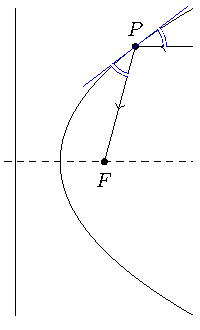
\includegraphics[width=\textwidth]{../Diagrams/Conics/parabola-cropped.pdf}
      \caption{A parabola.}
      \label{fig:parabola2}
    \end{subfigure}\hspace{0.1\textwidth}
    \begin{subfigure}{0.45\textwidth}
        \centering
        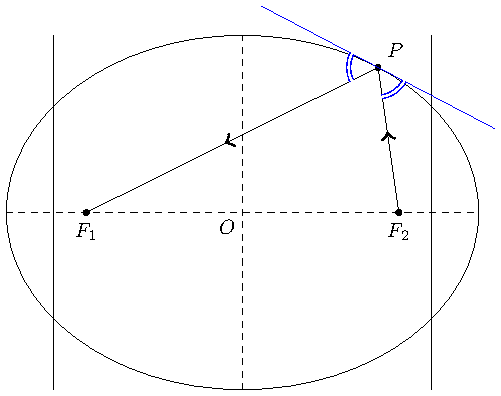
\includegraphics[width=\textwidth]{../Diagrams/Conics/ellipse.pdf}
        \caption{An ellipse.}
        \label{fig:ellipse2}
    \end{subfigure}

    \begin{subfigure}{0.45\textwidth}
      \centering
      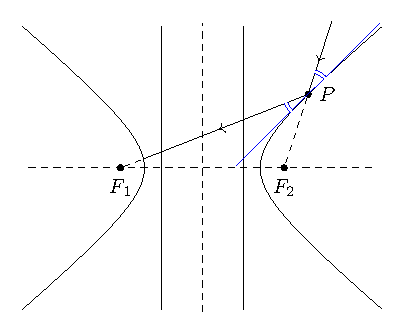
\includegraphics[width=\textwidth]{../Diagrams/Conics/hyperbola.pdf}
      \caption{A hyperbola}
      \label{fig:hyperbola2}
  \end{subfigure}
    \caption{\ref{Me} \ref{source:conics2} The reflective property of conics, their directrices, and foci.}
    \label{fig:conics2}
  \end{figure}
  \begin{itemize}[label=\(\circ\)]
    \item Conics in polar forms. Consider a conic with a focus at the origin, and a directrix 
  \end{itemize}
  \begin{table}[H]
    \centering
    \begin{tabular}{p{1.5cm}p{1.5cm}p{1.5cm}}
      & \begin{tabular}{|p{1.5cm}|}
        \hline
        \centering Top\\
        \(y=p\)
      \end{tabular} &\\
      \begin{tabular}{|p{1.5cm}}
        \hline
        \centering Left\\
        \(x=-p\)
      \end{tabular} &
      \begin{tabular}{|p{1.5cm}|}
        \hline
        \centering \vphantom{Top}\\
        \(\vphantom{y=p}\)
      \end{tabular} & 
      \begin{tabular}{p{1.5cm}|}
        \hline
        \centering Right\\
        \(x=p\)
      \end{tabular}\\
      \begin{tabular}{p{1.5cm}}
        \hline
        \centering \vphantom{Top}\\
        \(\vphantom{y=p}\)
      \end{tabular} &
      \begin{tabular}{|p{1.5cm}|}
        \hline
        \centering Bottom\\
        \(y=-p\)
      \end{tabular}
      & 
      \begin{tabular}{p{1.5cm}}
        \hline
        \centering \vphantom{Top}\\
        \(\vphantom{y=p}\)
      \end{tabular}\\
      & \begin{tabular}{p{1.5cm}}
        \hline \hphantom{1}   
      \end{tabular} &
    \end{tabular}
  \end{table}
  for some \(p>0\). In each respective case, the polar equation for the conic is given by
  \begin{table}[H]
    \centering
    \begin{tabular}{p{3cm}p{3cm}p{3cm}}
      & \begin{tabular}{|p{3cm}|}
        \hline
        \centering Top\\
        \[r=\frac{ep}{1+e\sin(\theta)}\]
      \end{tabular} &\\
      \begin{tabular}{|p{3cm}}
        \hline
        \centering Left\\
        \[r=\frac{ep}{1-e\cos(\theta)}\]
      \end{tabular} &
      \begin{tabular}{|p{3cm}|}
        \hline
        \centering \vphantom{Top}\\
        \[\vphantom{r=\frac{ep}{1+e\sin(\theta)}}\]
      \end{tabular} & 
      \begin{tabular}{p{3cm}|}
        \hline
        \centering Right\\
        \[r=\frac{ep}{1+e\cos(\theta)}\]
      \end{tabular}\\
      \begin{tabular}{p{3cm}}
        \hline
        \centering \vphantom{Top}\\
        \[\vphantom{r=\frac{ep}{1+e\sin(\theta)}}\]
      \end{tabular} &
      \begin{tabular}{|p{3cm}|}
        \hline
        \centering Bottom\\
        \[r=\frac{ep}{1-e\sin(\theta)}\]
      \end{tabular}
      & 
      \begin{tabular}{p{3cm}}
        \hline
        \centering \vphantom{Top}\\
        \[\vphantom{r=\frac{ep}{1+e\sin(\theta)}}\]
      \end{tabular}\\
      & \begin{tabular}{p{3cm}}
        \hline \hphantom{1}   
      \end{tabular} &
    \end{tabular}
  \end{table}
\end{stbox}
\begin{GCSkills}{}
  The parametric forms of the various conics can be found within the GC; no memorisation is needed!
  \begin{center}
    \texttt{apps} \(\Longrightarrow\) \texttt{2:Conics} \(\Longrightarrow\) \texttt{mode} \(\Longrightarrow\)  \texttt{PAR} \(\Longrightarrow\) \texttt{y=} \(\Longrightarrow\) 
    \begin{tabular}{Sc}
      \texttt{1:CIRCLE}\\
      \texttt{2:ELLIPSE}\\
      \texttt{3:HYPERBOLA}\\
      \texttt{4:PARABOLA}
    \end{tabular}.
  \end{center}
\end{GCSkills}
  \begin{note}
    \begin{itemize}[label=\(\circ\)]
      \item The area of an ellipse is given by \(\pi ab\).
      \item The \emph{major/minor axes} of an ellipse refer to the longest/shortest diameter of the ellipse. 
      \item The \emph{semi-major/semi-minor axes} of an ellipse refer to the longest/shortest radius of the ellipse. 
      \item A \emph{focal radius} of a conic is the distance from a point on the conic to a focus of the conic.
    \end{itemize}
  \end{note}
  \begin{note}
    Some possible things to try:
    \begin{itemize}
      \item Using \(PF_1+PF_2=2a\) to form simultaneous equations.
      \item Finding the polar form of a given conic (when \(e<1\) so \(r \geq 0\)) to solve for distances.
      \item Congruent/Similar triangles.
      \item Classic use of discriminants.
      \item \hyperlink{vieta}{Vieta's formula}.
    \end{itemize}
  \end{note}
  \begin{example}{}{}
    Describe the significance of the reflective property of parabolas in relation to the reception of the satellite TV.
    \begin{itemize}
      \item As the satellite is very far from the parabolic dish, the rays coming towards the dish can be taken to be parallel rays.
      \item These rays would all be reflected by the dish and converge at the focus. So, the receiver so should be placed at the focus to maximise the reception of the satellite TV. 
    \end{itemize}
  \end{example}